\chapter{Implementación}

En este capítulo se va a proceder a desarrollar cada uno de los PMV de cara a cada hito relacionado con 
la implementación, ya que los hitos previos \footnote{\url{https://github.com/JoseJordanF/Claqueta/milestone/1}} 
\footnote{\url{https://github.com/JoseJordanF/Claqueta/milestone/7}} se encuentran en el capítulo de 
planificación, ya que definen la infraestructura y organización del proyecto. Además, habrá que 
discutir que herramientas van a usarse para desarrollar o llevar a cabo estos hitos y el porqué de su 
elección. 

Dividiéndose la implementación del software en hitos. Estos han sido definidos en Github
y cada uno de ellos contiene un grupo de \textit{issues} que se corresponden con las distintas
mejoras que se han ido incorporando al software a lo largo de su desarrollo.

El uso de herramientas permiten llevar a cabo el proyecto, asegurando su calidad y buenas prácticas 
durante el uso de estas.

Por ello se van a describir las herramientas principales que se van a utilizar para el desarrollo 
del software, en cada uno de los hitos. Describiendo los lenguajes de programación que se usaran, 
lenguajes de consulta y manipulación de datos para API, el modelo de datos a usar, a su vez también 
se mostraran herramientas que velen por el buen desarrollo en el repositorio y llevar a cabo buenas 
prácticas. El uso de todas estas herramientas será justificado, explicándose así para qué se va a 
utilizar dicha herramienta y porque se ha elegido.

\section{M1: Definición de objetos - Abstracción del dominio del problema}

En este hito \footnote{\url{https://github.com/JoseJordanF/Claqueta/milestone/8}} se conseguirá el 
modelado de los objetos presentes en el problema, para ello se abstraerán 
los conceptos clave y se definirán los objetos de la aplicación. El objetivo es tener una estructura 
clara de los datos a utilizar. La abstracción nos permite identificar las características 
esenciales, eliminando detalles innecesarios. La definición de objetos nos ayudará a comprender sus 
relaciones, atributos y operaciones. Esto establecerá una base sólida para el desarrollo coherente 
de la aplicación.

De esta manera se busca priorizar el desarrollo real, la retroalimentación continua y prácticas como 
el desarrollo impulsado por pruebas \begin{otherlanguage}{english}\textit{(Test Driven Development, TDD)}\end{otherlanguage}  ,y la colaboración cercana. Esto permite una mayor 
agilidad y adaptabilidad en el proceso de desarrollo.

Por ello, buscando un método para definir los objetos de la aplicación, se encuentra una técnica de 
desarrollo de software llamada, \begin{otherlanguage}
{english}``\textit{\textbf{Domain Driven Design}}''\end{otherlanguage}(DDD) \cite{NvDDD} es un enfoque 
de diseño de software que se centra en comprender y modelar el dominio del problema de una aplicación. 
Busca desarrollar un diseño que refleje con precisión las reglas y conceptos del dominio, lo que 
resulta en un sistema más mantenible. Teniendo en cuenta que el DDD y el desarrollo ágil son 
compatibles, ya que su aplicación permite construir aplicaciones que se ajusten mejor a las necesidades 
del cliente y evolucionen de manera flexible a medida que se adquiere un mayor entendimiento del 
dominio. DDD proporciona la base conceptual y un diseño sólido para desarrollar modelos de dominio 
claros y significativos, mientras que el enfoque ágil permite una implementación iterativa, rápida y 
adaptativa.

De esta manera se recurre al uso del \textit{\textbf{modelo de dominio}} representación conceptual de 
las entidades, los conceptos, las reglas, objetos inmutables, como los objetos valor y las 
interacciones dentro del dominio del problema. Es una abstracción del mundo real que captura las 
principales entidades y sus relaciones. Esto ofrece una gran ventaja del DDD, ya que esto ayuda a 
alinear el entendimiento y facilita la comunicación efectiva sobre el problema y su solución. Siendo 
los modelos de dominio una parte central y fundamental del DDD, representando el conocimiento y la 
comprensión profunda del problema que se está abordando. Teniendo esto en cuenta se crea un modelo de 
dominio.

\begin{figure}[h]
    \centering
    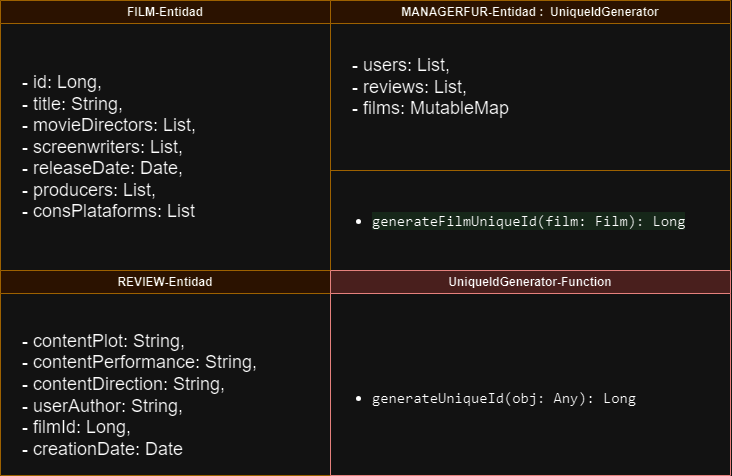
\includegraphics[width=\linewidth]{imagenes/Modelo_Dominio_Claqueta_TFG.drawio.png}
    \caption{Modelo de dominio.}
    \label{fig:diagrama}
\end{figure}



Como base y resumen del modelo de dominio, tendríamos una entidad \begin{otherlanguage}
{english}\textit{\textbf{review }}\end{otherlanguage}haciendo referencia a la reseña, la entidad 
esencial, ya que perseguimos asegurar la calidad de esta. Una reseña de calidad va a ser definida 
comúnmente como una reseña fiable que cumpla las reglas que vimos en el estado del arte. Por lo tanto, 
tendremos atributos generales como el autor de la reseña, un identificador que la relacione con la 
película a la cual está criticando, la fecha de realización de esta crítica y también el 
contenido de la reseña se dividiría para que el usuario hable tanto de la trama general, la 
interpretación y la dirección. Asegurando las reglas vistas en el estado del arte.

Otra entidad importante es la \begin{otherlanguage}{english}\textit{\textbf{film }}\end{otherlanguage} 
siendo su propuesta mínima un conjunto de atributos que definen el contenido de dicha película como los 
directores, los guionistas, la fecha de estreno, las productoras y las plataformas en las que se puede 
consumir dicha película. Este conjunto de atributos es indispensable para la recomendación de dicho 
contenido, siendo cada uno puntos en común que buscar en otras películas para sus recomendaciones 
personalizadas según su contenido. Evidentemente, también necesitamos el título de la película y un 
identificador, ya que el resto de atributos puede coincidir y no identificar de manera única a la 
película.

Por último, tenemos una entidad que se encarga de gestionar tanto películas, como reseñas, como 
usuarios. Además, implementa la interfaz que nos permitirá generar el identificador único para cada 
película.

\subsection{Lenguaje de programación}

Una de las principales herramientas para el desarrollo de software es el lenguaje de programación, un 
lenguaje que sea afín a las necesidades del proyecto. Siendo así un necesario un lenguaje para modelar 
los objetos descritos en este capítulo, en el primer hito. Pero debemos tener en cuenta que se pretende 
que el desarrollo del modelado de los objetos pueda ser reutilizable, de fácil acceso e intentando 
ahorrar recursos. Por ello, para la aplicación es posible crear una API propia, como las que se 
mencionaron en el capítulo del estado del arte. Ya que es muy atractivo que los algoritmos y el modelo 
de datos pueda ser consumido por otros a través de una API

Por ahora deberíamos encontrar un lenguaje que sea flexible y que se adapte a nuestras necesidades. Con 
lo que buscamos un lenguaje de propósito general, lo cual nos permitirá crear diversos proyectos. 
Siendo estos más sencillos de implementar en unos lenguajes que en otros. Podríamos pensar en lenguajes 
como Java, Groovy, Scala o Kotlin. Siendo todos ejecutados en la máquina virtual de java (JVM), siendo 
Java, el veterano, es robusto y multiplataforma, pero su sintaxis puede ser un tanto prolija. Kotlin, 
por su parte, destaca por ser moderno, conciso y compatible con Java, además de ofrecer avanzadas 
características de seguridad. Aunque Groovy simplifica la sintaxis, su velocidad de ejecución más lenta 
podría ser un inconveniente. Scala, con un enfoque en la programación funcional, es expresivo, pero 
puede presentar una curva de aprendizaje más pronunciada. En conclusión, Kotlin emerge como la elección 
óptima en la JVM debido a su curva de aprendizaje suave, su amplia gama de bibliotecas y su excepcional 
interoperabilidad con Java, presentando una combinación equilibrada de simplicidad y funcionalidades 
avanzadas. Siendo bastante atractivo la posibilidad de hacer aplicaciones móviles nativas, punto a 
tratar cuando concluyamos que tipo de aplicación vamos a desarrollar.

Por otro lado, necesitaremos un flujo de trabajo que nos permita comprobar la calidad del código escrito en dicho 
lenguaje. Cada cambio, cada nueva incorporación al código, se debe asegurar su calidad. Para ello se busca un lint para
Kotlin, que asegure la corrección y calidad del código. Para ello primero debemos elegir un sistema de integración 
continua para llevar a cabo este flujo de trabajo. Por lo que debemos establecer que buscamos en un sistema de CI, en 
primer lugar, se debe asegurar la compatibilidad con Kotlin, garantizando que el CI pueda ejecutar tareas específicas 
para este lenguaje, como el análisis estático de código (lint). Además, es esencial verificar la integración fluida con 
GitHub, permitiendo la configuración de flujos de trabajo basados en eventos del repositorio. La automatización de tareas 
de lint debe ser admitida, abarcando la ejecución de herramientas de análisis estático de código para identificar y 
corregir problemas de estilo y calidad. La personalización de flujos de trabajo es clave, buscando un CI que ofrezca 
flexibilidad para integrar pasos específicos relacionados con el análisis de código. La capacidad de recibir 
notificaciones inmediatas sobre los resultados del análisis de código facilitará una retroalimentación rápida. Considerar 
también el soporte de contenedores para simplificar la configuración del entorno de ejecución. La escalabilidad del 
sistema de CI es esencial, asegurándose de que pueda manejar proyectos de diferentes tamaños eficientemente. La capacidad 
de rastrear y analizar el historial de ejecución de flujos de trabajo es crucial para evaluar la consistencia y mejorar 
continuamente dicho flujo. La seguridad, tanto en la protección de resultados de análisis de código como en la gestión de 
credenciales. Por último, se debe considerar el modelo de costos y licenciamiento del CI para asegurar que se ajuste al 
presupuesto del proyecto.

De esta manera pasemos a sopesar varias opciones \cite{BestCI} como \textbf{Jenkins}:
\begin{itemize}
  \item \textbf{Compatibilidad con Kotlin:} Jenkins es altamente extensible y tiene soporte para Kotlin a través de 
  plugins. Puedes utilizar el plugin ''Kotlin'' para ejecutar tareas específicas para este lenguaje.
  \item \textbf{Integración con GitHub:} Jenkins se integra bien con GitHub mediante plugins como ''GitHub Integration'' 
  y ''GitHub Branch Source'', permitiendo configurar flujos de trabajo basados en eventos de GitHub.
  \item \textbf{Automatización de Tareas de lint:} Puedes configurar pasos específicos de lint en Jenkins utilizando 
  scripts y plugins relevantes para análisis estático de código en proyectos Kotlin.
  \item \textbf{Personalización de Flujos de Trabajo:} Jenkins es conocido por su flexibilidad y capacidad de 
  personalización. Puedes definir flujos de trabajo complejos y personalizados según tus necesidades específicas.
  \item \textbf{Notificaciones y Retroalimentación:} Jenkins proporciona opciones para notificar resultados de manera 
  inmediata a través de integraciones con servicios como Slack o correo electrónico.
  \item \textbf{Soporte de Contenedores:} Jenkins es compatible con contenedores a través de plugins como ''Docker 
  Pipeline'' y ''Kubernetes Continuous Deploy''.
  \item \textbf{Escalabilidad:} Jenkins es escalable y se puede configurar para manejar proyectos de diferentes tamaños y 
  complejidades.
  \item \textbf{Historial y Trazabilidad:} Jenkins mantiene un historial detallado de ejecuciones de trabajos, 
  proporcionando trazabilidad y permitiendo el análisis de resultados anteriores.
  \item \textbf{Seguridad:} Jenkins tiene funcionalidades de seguridad robustas, incluyendo opciones para gestionar 
  credenciales de forma segura y configurar permisos a nivel de proyecto.
  \item \textbf{Costo y Licenciamiento:} Jenkins es de código abierto y gratuito, lo que lo hace una opción rentable. Sin 
  embargo, es posible que la implementación y mantenimiento pueden requerir recursos como hardware o extensiones 
  adicionales.
\end{itemize}

En resumen, Jenkins cumple con muchos de los criterios necesarios para ejecutar tareas de lint en proyectos Kotlin, 
brindando flexibilidad y personalización, aunque su configuración y administración pueden ser más complejas en 
comparación con algunas soluciones más modernas.

Otra opción podría ser \textbf{GitLab CI}:
\begin{itemize}
  \item \textbf{Compatibilidad con Kotlin:} GitLab CI admite la ejecución de tareas específicas de Kotlin, incluyendo 
  linters y otras herramientas de análisis estático de código.
  \item \textbf{Integración con GitHub:} Aunque el repositorio esté en GitHub, GitLab CI puede integrarse y ejecutarse 
  sin problemas mediante configuraciones específicas y desencadenadores webhook.
  \item \textbf{Automatización de Tareas de lint:} GitLab CI permite definir pasos específicos para ejecutar linters y 
  otras herramientas de análisis estático como parte de un flujo de trabajo.
   \item \textbf{Personalización de Flujos de Trabajo:} GitLab CI utiliza archivos \texttt{.gitlab-ci.yml} para definir 
   flujos de trabajo, lo que facilita la configuración y personalización de tareas de lint.
  \item \textbf{Notificaciones y Retroalimentación:} GitLab CI proporciona opciones para notificar sobre el estado de los 
  flujos de trabajo, integrándose con servicios como Slack o correo electrónico.
  \item \textbf{Soporte de Contenedores:} GitLab CI admite la ejecución de flujos de trabajo en diversos ejecutores, 
  incluyendo máquinas virtuales, contenedores Docker y ejecutores compartidos.
  \item \textbf{Escalabilidad:} GitLab CI se adapta a proyectos de diversos tamaños y complejidades, permitiendo la 
  ejecución de flujos de trabajo en paralelo.
  \item \textbf{Historial y Trazabilidad:} GitLab CI mantiene un historial detallado de ejecuciones de flujos de trabajo,
  permitiendo la revisión de resultados anteriores y proporcionando trazabilidad completa.
  \item \textbf{Seguridad:} GitLab CI ofrece opciones para gestionar secretos y credenciales de manera segura, siguiendo 
  prácticas de seguridad recomendadas.
  \item \textbf{Costo y Licenciamiento:} GitLab CI es parte integral de GitLab, que ofrece una versión gratuita con 
  funciones básicas, así como opciones de licenciamiento para funcionalidades avanzadas y soporte empresarial.
\end{itemize}

Y otra de las mejores herramientas de integración continua como \textbf{GitHub Actions}:

\begin{itemize}
  \item \textbf{Compatibilidad con Kotlin:} GitHub Actions es versátil y admite fácilmente proyectos Kotlin. Puedes
  utilizar acciones y configuraciones específicas para ejecutar tareas de lint en código Kotlin.
  \item \textbf{Integración Profunda con GitHub:} GitHub Actions está estrechamente integrado con GitHub, facilitando la 
  configuración de flujos de trabajo basados en eventos específicos de GitHub, como push o pull requests.
  \item \textbf{Automatización de Tareas de lint:} GitHub Actions permite definir pasos personalizados para ejecutar 
  herramientas de análisis estático de código, incluidos los linters para Kotlin.
  \item \textbf{Personalización de Flujos de Trabajo:} Puedes personalizar fácilmente flujos de trabajo en GitHub Actions 
  según tus necesidades, definiendo pasos y acciones específicas para el análisis de código.
  \item \textbf{Notificaciones y Retroalimentación:} GitHub Actions ofrece integración nativa con notificaciones de 
  GitHub, Slack, y otras plataformas, proporcionando retroalimentación inmediata sobre los resultados de los flujos de 
  trabajo.
  \item \textbf{Soporte de Contenedores:} GitHub Actions incluye soporte nativo para contenedores Docker, lo que facilita 
  la ejecución de tareas en entornos específicos.
  \item \textbf{Escalabilidad:} GitHub Actions se escala automáticamente según la demanda, lo que lo hace adecuado para 
  proyectos de diversos tamaños y complejidades.
  \item \textbf{Historial y Trazabilidad:} GitHub Actions mantiene un historial detallado de ejecuciones de flujos de 
  trabajo, permitiendo la revisión de resultados anteriores y proporcionando trazabilidad completa.
  \item \textbf{Seguridad:} GitHub Actions sigue los protocolos de seguridad de GitHub y proporciona opciones para 
  gestionar secretos y credenciales de forma segura.
  \item \textbf{Costo y Licenciamiento:} GitHub Actions ofrece una cantidad gratuita de minutos para ejecutar flujos de
  trabajo, y los precios adicionales son proporcionales al uso. El modelo de precios es transparente y basado en el 
  consumo real.
\end{itemize}

En resumen, GitHub Actions es una solución integral que cumple con los requisitos de ejecución de tareas de lint en 
proyectos Kotlin, proporcionando una integración profunda con GitHub y una experiencia más moderna y sencilla en 
comparación con sistemas más antiguos como Jenkins. GitLab CI es una opción sólida para ejecutar tareas de lint en 
proyectos Kotlin en GitHub, proporcionando flexibilidad, integración y un conjunto de características completo. Sin 
embargo, la estrecha integración de GitHub Actions y la accesibilidad a la retroalimentación y la comodidad de usarlo en 
la propia plataforma prevalecen sobre GitLab CI, ya que son herramientas bastante similares, nos aferramos a estos 
últimos atributos para terminar con la eleccion de GitHub Actions como sistema de CI para nuestro lint.

\subsection{Persistencia de datos}

La persistencia de datos es primordial para realizar cualquier lógica de negocio. Necesitamos tanto 
datos del usuario como las entidades que representan los objetos con los que interactúan estos 
usuarios. Para ello necesitamos una base de datos, en Kotlin poseemos una gran variedad de opciones. Por 
ejemplo, opciones sencillas de usar y generalmente rápidas como las bases de datos clave-valor, como Firebase 
Database, Redis, Cassandra y LevelDB, ofrecen soluciones para una amplia gama de aplicaciones. Firebase 
Database es ideal para aplicaciones web y móviles que necesitan sincronización en tiempo real. Redis 
sobresale en almacenamiento en memoria y caché, permitiendo la manipulación de varios tipos de datos y 
brindando una rápida recuperación. Cassandra se destaca en la escalabilidad horizontal y la alta 
disponibilidad, adecuada para grandes volúmenes de datos. LevelDB ofrece un almacenamiento eficiente en 
disco. Sin embargo, la elección se inclina hacia Redis, gracias a su capacidad para almacenar datos flexibles 
y variables, y a su facilidad para manejar diversos tipos de estructuras de datos como las vistas en modelo 
de dominó. La curva de aprendizaje es baja para Firebase Database, Redis y LevelDB, mientras que Cassandra 
puede requerir una mayor comprensión de conceptos distribuidos y esquemas de datos más complejos.

También nos podemos apoyar en como se nos indica \cite{NosqlDist}, como podríamos elegir una base de datos 
NoSQL, mencionando como las bases de datos clave-valor son excelentes para datos simples y estructuras 
básicas, adaptándose bastante bien estos modelos de datos. Siendo idóneas para almacenar información de 
sesión o datos en caché, convirtiéndose en una opción sólida si buscamos alta disponibilidad, dado su rápido 
acceso a través de claves, y una escalabilidad horizontal.


\subsection{Inyección de dependencias}


La inyección de dependencias es esencial en proyectos de software \cite{DIart}\cite{BenDI} para 
promover la modularidad y la reutilización del código. Permite desacoplar componentes, lo que facilita 
las pruebas unitarias y el mantenimiento. Al separar la creación de objetos de su uso, se logra una 
mayor flexibilidad y extensibilidad del sistema, lo que facilita la incorporación de nuevas 
funcionalidades sin afectar el código existente. En resumen, la inyección de dependencias promueve un 
diseño limpio y eficiente en el desarrollo de software.

En el mundo de Kotlin, existen varias opciones para facilitar la inyección de dependencias en tus 
proyectos. Koin destaca por su simplicidad y se integra de manera natural con aplicaciones Android. 
Dagger 2, una biblioteca de Google, se basa en anotaciones y brinda una inyección de dependencias 
eficiente y segura, ideal para proyectos extensos. Hilt, una extensión de Dagger 2, simplifica la 
inyección de dependencias en aplicaciones Android, lo que la hace atractiva para desarrolladores 
móviles. Ya que no es un proyecto muy extenso, la opción estaría entre Koin y Hilt. Ambas son buenas 
opciones, sin embargo, Koin es conocido por su enfoque sencillo y sintaxis intuitiva, lo que lo hace 
ideal para proyectos pequeños o si buscas una curva de aprendizaje suave. Por estos dos motivos, Koin 
será la opción seleccionada para llevar a cabo la inyección de dependencias.

\subsection{Testing}

Un proyecto con un enfoque ágil está sujeto a pruebas constantemente, algo que estamos apegando en este 
proyecto a los PMVs resultantes de los milestones. Como ya sabemos de esta manera, aseguramos la 
calidad del producto y nos cerciora de que todo funciona como debería. Consiguiendo así productos de 
calidad más robustos minimizando errores.

Como hemos mencionado, Kotlin goza de acceso a un extenso conjunto de librerías y \textit{frameworks}. 
En este conjunto existen varios \textit{frameworks} que nos permiten testear nuestro código.

Una herramienta esencial para fortalecer el proceso de desarrollo, las pruebas de flujo de trabajo con Docker 
\cite{GI_act}. Esta herramienta nos permite llevar a cabo pruebas exhaustivas de los flujos de trabajo de manera 
local antes de su implementación en el entorno remoto, destacándose por su integración efectiva con Docker. La 
característica distintiva de esta herramienta radica en dicha capacidad para generar simulaciones precisas, 
lanzando y evaluando flujos de trabajo en un entorno controlado basado en Docker. Asegurando la funcionalidad y 
consistencia de los flujos de trabajo antes de su inclusión en el entorno remoto, proporcionando la confianza 
necesaria en la calidad del código. Siendo una herramienta clave para garantizar una implementación sin 
contratiempos, mejorando la robustez y la calidad de los flujos de trabajo antes su despliegue.

Para test unitarios del código encontramos varios \textit{frameworks}, por un lado, tenemos 
\textit{Spek}\footnote{\url{https://github.com/spekframework/spek}}. Una herramienta escrita para 
Kotlin diseñado para facilitar la escritura y ejecución de pruebas en proyectos escritos en este 
lenguaje. Permite definir pruebas en un estilo legible similar al lenguaje natural, lo que facilita 
su comprensión tanto para desarrolladores como para no desarrolladores. Por ello, algunos 
desarrolladores lo relacionan con \begin{otherlanguage}
{english}\textit{Behavior-Driven Development}\end{otherlanguage} (BDD), desarrollo guiado por 
comportamiento. Aunque sus creadores ya han mencionado 
\footnote{\url{https://spekframework.github.io/spek/docs/latest/}} que creen que hay una falsa 
distinción en torno al desarrollo guiado por comportamiento (BDD) y desarrollo guiado por pruebas 
(TDD). Por lo que recomiendan que pensemos en Spek como un simple \textit{framework} de 
especificación.

También disponemos de la herramienta por defecto que incorpora cualquier tipo de proyecto Kotlin, 
\textit{JUnit5}. Este es la última versión del \textit{framework} de pruebas unitarias para Java. Posee 
una arquitectura modular que se compone de tres módulos principales: JUnit Platform, JUnit Jupiter y 
JUnit Vintage, el primero es el núcleo de la herramienta, el segundo introduce las anotaciones y 
permite configurar los test, y la última permite la compatibilidad con versiones anteriores de este 
\textit{framework}. Este es el más usado actualmente por los desarrolladores Android 
\footnote{\url{https://www.jetbrains.com/es-es/lp/devecosystem-2022/testing/}} como nos indica 
\textbf{\textit{Jetbrains}}, compañía que ha diseñado Kotlin.

Ambos son buenas herramientas de pruebas. Además, permiten la integración con otras bibliotecas o 
\textit{framework} de pruebas. Pero ambas herramientas necesitan de otras bibliotecas imprescindibles 
en las pruebas, estas permiten simular objetos de una clase para trucar el resultado de ciertas 
funciones que queremos testear. Estos objetos se denominan \textbf{\textit{Mock}}, en Kotlin 
encontramos la librería nativa \textit{mockk}. Con el par de uno de los \textit{frameworks} 
mencionados y esta librería podríamos realizar los test unitarios que necesitemos. Pero principalmente 
si no en su totalidad usaremos Junit5 debido a la cantidad de información y ejemplos de uso, además de 
ser la usada por la mayoría de desarrolladores Android.

Para la parte de testeo de UI tenemos acceso a varias herramientas, pero nos limitaremos a usar el 
\textit{framework} \textbf{\textit{Espresso}}\footnote{\url{https://developer.android.com/training/testing/espresso?hl=es-419}}, una herramienta creada por Google y la más recomendada \cite{UITest}.

Por último, si fuera necesaria una herramienta para testear las operaciones de una API, si es que 
decidimos crearla, para  recuperar, insertar, modificar o eliminar información. Como hemos visto entre 
las herramientas más usadas para las pruebas\footnote{\url{https://www.jetbrains.com/es-es/lp/devecosystem-2022/testing/}} se encuentra \textit{\textbf{Postman}} una página para ayudar a los 
desarrolladores de API. Por ello es la herramienta que usaremos en tal caso para realizar dichas 
pruebas, además es sencilla y cómoda de usar.

\subsection{M2: Lógica de negocio - Operaciones sobre los datos}

En este hito \footnote{\url{https://github.com/JoseJordanF/Claqueta/milestone/3}} se hablará de la 
lógica de negocio, también conocida como reglas de negocio, se refiere a las operaciones y procesos 
fundamentales que definen cómo funciona la aplicación. Determinando como se procesan los datos, se 
realizan cálculos, se toman decisiones y se llevan a cabo las operaciones clave para lograr los 
objetivos de la aplicación. Siempre dependientes de las necesidades y los propósitos de la aplicación. 
Como estas vienen definidos por las \textbf{Historias de Usuario}, vamos a recurrir a ellas para 
determinar las operaciones que se llevaran a cabo con los datos. Aseguraremos la correcta 
implementación de la lógica de negocio, asegurando la coherencia y validez en las operaciones a través 
de los test unitarios. siguiendo como siempre la esencia del desarrollo ágil, debemos asegurar las
buenas prácticas y garantizar la calidad del proyecto, teniendo en cuenta que la lógica de negocio es 
el núcleo esencial que da vida a una aplicación y hace posible su funcionalidad y utilidad. 

Cabe destacar que lo primero que se hará es crear un proyecto Kotlin creado por gradle, un sistema de 
automatización de construcción de código de software por defecto, en este caso en IntelliJ IDEA. Esto 
es imprescindible, ya que para una mayor comodidad en la configuración y el uso de las distintas 
herramientas que nos ofrece Kotlin es necesario la creación de un proyecto.
Cada una de las siguientes secciones representa un conjunto de issues que se han resuelto para obtener 
un pmv.

\subsubsection{Identificación y creación de las películas}

Una vez creado el proyecto con nuestros modelos de dominio, estamos listos para comenzar con las 
distintas operaciones sobre los datos. Para empezar nos deberíamos preguntar qué contenido van a 
consumir los usuarios, claramente películas y en sí las reseñas de estas. Por lo tanto, primeramente 
deberíamos diferenciar de manera única cada película. Para ello tenemos el identificador de cada 
película, pero aún no hemos definido como se creara dicho identificador. Para generar este 
identificador podemos optar por múltiples opciones, se podría pensar que usar el título de la película 
o el nombre de alguno de los directores sería buena idea. Pero esto nos lleva a un problema debido a 
que nos encontramos películas que poseen el mismo título y son diferentes, al igual que los directores. 
Incluso por eso se puede llegar a dar la casualidad de que existan dos películas con el mismo título y 
un director en común, siendo estas diferentes. Por lo tanto, no podríamos usar el título y algún 
director, o al menos si solo usamos estos datos. Por lo tanto, esta deja de ser una posibilidad, aun 
así tenemos muchas más opciones, podríamos recurrir a la base de datos para generar un identificador 
único, ya que muchas bases de datos modernas poseen esta función incorporada. Pero no se quiere 
depender de la base de datos para generar estos identificadores, ya que en este punto del proyecto no 
es necesaria la base de datos. De manera que existen otras opciones como GUID una implementación de 
Windows para generar identificadores siguiendo un algoritmo específico, o alguna otra opción como los 
métodos que usan una marca en el tiempo y un identificador para cada nodo en el sistema. La comparación 
entre ambas opciones \cite{compSnowUUID} nos deja que las opciones estilo UUID son valores de 128 bits 
y no tienen un criterio determinado para generar dicho identificador, mientras que los métodos estilo 
snowflake son valores enteros de 64 bits y tienen una forma determinada de generar dicho identificador. 
debido a la facilidad de seguir un algoritmo determinado y que no necesitamos representar demasiados 
datos como para usar 128 bits, se ha decidido usar snowflake \cite{snowF} método creado por Twitter. 
Básicamente, se basa en crear un identificador único representando en decimal un número binario creado 
por bloques, el primero de 41 bits que define los milisegundos pasados desde una marca de tiempo 
determinada, el segundo bloque de 10 bits representa un identificador propio del objeto, en este caso 
se ha decidido fusionar el título de la película y el nombre del primer director para crear un número 
de 10 bits para este bloque. Por último, el bloque final de 12 bits que simplemente represente un 
número de secuencia por si se da la casualidad que se crean varios objetos en el mismo milisegundo y 
con el mismo título y primer director. Dándonos un identificador que cumple con nuestras necesidades de 
sobra.

\subsubsection{Que es el consumo, quién lo consume y como lo lleva a cabo}

Tras resolver este problema para identificar el contenido, podemos pasar a definir como crear ese 
contenido por parte de la entidad que administra todo. Para ello, cada vez que se crea una película, 
además de introducir todos los datos requeridos, se crea su identificador y se añade a la lista de 
películas del proyecto. Ahora bien, para que este contenido pueda ser consumido por los usuarios dichos 
usuarios deben estar creados en el sistema, por tanto, definimos como se crea un usuario y se introduce 
en la lista de usuarios. Esto nos lleva a responder como definimos el consumo y como designamos que un 
usuario ha consumido, en este caso una película. Lo que nos lleva a una interacción por parte del 
usuario para responder a esas preguntas, a primera vista definimos el consumo, la interacción del 
usuario como la creación de reseñas por parte de este. Siendo las películas en las que reseña o en las 
que interactúa con las reseñas de alguna manera, las películas que consume el usuario. Esto es algo que 
se definirá más adelante en la lógica de negocio. 

\subsubsection{Creación de reseñas}

Una vez creadas las películas y los usuarios, necesitamos definir como se crean las reseñas a través de 
los datos necesarios, la relación con la película y el usuario que la ha escrito. Ya que tenemos todo 
lo necesario para la creación de esta reseña. Dando lugar a la reseña en sí misma y a la marca del 
consumo por parte del usuario, tema mencionado justo en la sección anterior. Además de comprobar que no 
exista una reseña de esa película ya escrita por este usuario, ya que cada usuario solo puede escribir 
una reseña por película.

\subsubsection{Recomendación de contenido al usuario}

Definido el consumo como la realización de reseñas es las distintas películas, tomamos esto como marca 
de consumo como se mencionaba en la creación de reseñas. De esta manera conseguimos el consumo del 
usuario, siendo este todas las películas en las que ha reseñado el usuario. Y siendo las películas 
elegidas para recomendar consumo a este. Las recomendaciones se harán a través de los datos comunes de 
estas películas, los directores, las productoras, los guionistas o las plataformas donde se pueden ver 
estas películas. Cualquiera de estos datos se utilizará para recomendar cualquier película que no se 
haya consumido y tenga algún dato en común con el consumo del usuario. De esta manera tendríamos una 
lista de películas recomendadas para el usuario sin repetidos, ya que es posible que varios datos 
coincidan en las mismas películas. Esta lista se refrescará cada vez que el usuario escriba una reseña 
en una nueva película.

Por cada una de estas operaciones se pueden dar varios casos de uso que se han estudiado a través de 
los test unitarios. Comprobando que cada caso de uso se lleva a cabo como se espera y el conjunto de 
ellos también.
